\documentclass[tikz, border=15pt]{standalone}
\usepackage{tikz}
\usetikzlibrary{positioning, calc}

\begin{document}

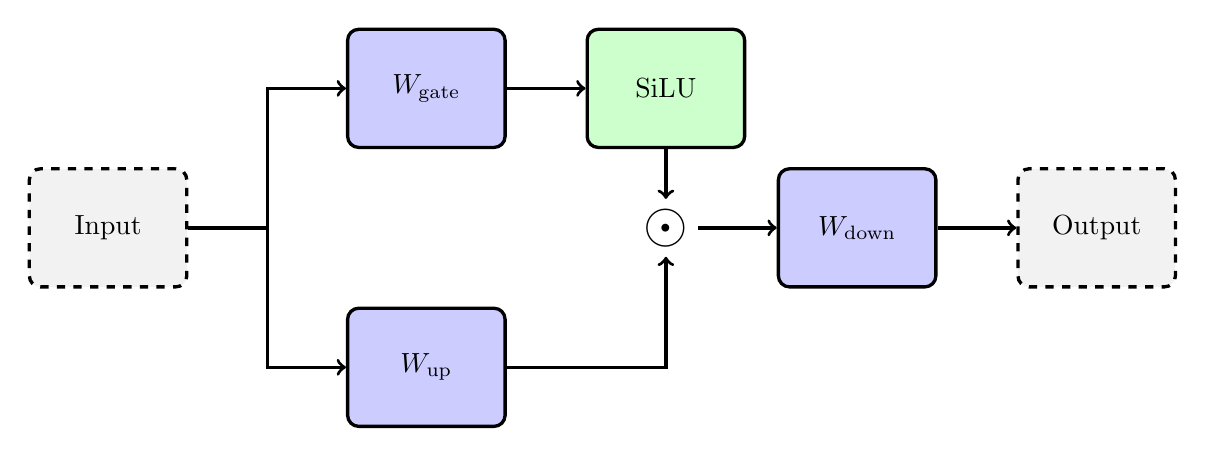
\begin{tikzpicture}[
    data/.style={
        draw,
        very thick,
        rounded corners,
        minimum width=2cm,
        minimum height=1.5cm,
        dashed,
        fill=gray!10, 
    },
    module/.style={
        draw,
        very thick,
        rounded corners,
        minimum width=2cm,
        minimum height=1.5cm,
    },
    weight/.style={
        module,
        fill=blue!20,
    },
    arrow/.style={
        ->,
        very thick,
    },
]

    \node[data] (input) {Input};
    \coordinate[right=of input] (split);
    \node[weight, above right=of split] (gate) {$W_{\mathrm{gate}}$};
    \node[weight, below right=of split] (up) {$W_{\mathrm{up}}$};
    \node[module, fill=green!20, right=of gate] (SiLU) {$\mathrm{SiLU}$};
    \node[font=\huge] (multiply) at ($(SiLU |- input)$) {$\odot$};
    \node[module, fill=blue!20, right=of multiply] (down) {$W_{\mathrm{down}}$};
    \node[data, right=of down] (output) {Output};

    \draw[very thick] (input) -- (split);
    \draw[arrow] (split) |- (gate);
    \draw[arrow] (split) |- (up);
    \draw[arrow] (gate) -- (SiLU);
    \draw[arrow] (up) -| (multiply);
    \draw[arrow] (SiLU) -- (multiply);
    \draw[arrow] (multiply) -- (down);
    \draw[arrow] (down) -- (output);

\end{tikzpicture}

\end{document}